\documentclass{article}
\usepackage{graphicx}
\usepackage{amsmath}
\usepackage{hyperref}
\usepackage{float}
\usepackage{xcolor}
\usepackage{enumitem}
\usepackage{hyperref}
\usepackage{mathtools}

\begin{document}

\title{Solutions to hw3 homework on Convex Optimization https://web.stanford.edu/class/ee364b/homework.html}
\author{Andrei Keino}
\maketitle

\section*{3.1 (4 points)} 
Consider the optimization problem

\begin{align*}
	minimize_{\{x_j\}_{j = 1}^J} \; &  
	f(x_1, \dots, x_j) \coloneqq
	\frac{1}{2} \lVert b - \sum_{j = 1}^{J} 
	A_j x_j \rVert_2^2 
	+ \lambda \cdot   \sum_{j = 1}^{J} 
	\lVert x_j \rVert_2,
	\\
	& s.t. \; A_j x_j \geq 0, \; \forall j 
	\in \{1, 2, \dots, J\} \\
\end{align*}
with variable $x_1, \dots, x_J \in R^n, $ and 
problem data $A_1, \dots, A_J \in R^{m \times n}, $ 
$b \in R^m,$ and $\lambda > 0.$ for constrained optimization given on page 11 (really p. 12) of the lecture slides for subgradient methods for constrained problems. \\

% file 
% C:\! Convex_Optimization\ConvexOptimizationII\materials\lsocoee364b/03-constr_subgrad_slides.pdf

Let $J = 3,$ $n = 100,$ $m = 10$ and $\lambda = 0.5$ Generate random matrices
$A_1, \dots , A_J \in R^{m\times n}$ with independent uniformly distributed entries in the interval 
$[0, \frac{1}{\sqrt{m}}),$ and, random vectors $x_1, \dots,  x_J \in 2 R^n$uniformly distributed entries in the interval 
$[0, \frac{1}{\sqrt{n}}),$ then set 
$b = \sum_{j = 1}^{J} A_j x_j.$
Plot convergence in terms of the
objective $f(x_1^{(k)}, \dots x_1^{(J)}).$ 
Try different step length schedules. Also, plot the maximal violation for the linear constraints at each step.\\

Solution: \\
\textbf{The code is in the file} \verb |solution_3_1_b.m.| The code 
is nearly the same as one for the task 2.4, the only difference that on every step of the gradient descent we are calculating the constraint violation vector and if 
there are at least one violation, we replace the gradient of the minimized function with the gradient of any constraint violation found.

\begin{figure}[H]
	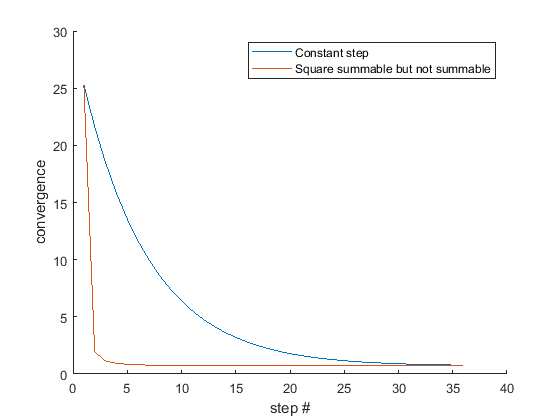
\includegraphics[width=\linewidth]{fig_3_1_1.png}
	\caption{Convergence with different step length.}
	\label{fig:3_1_1}
\end{figure}

\begin{figure}[H]
	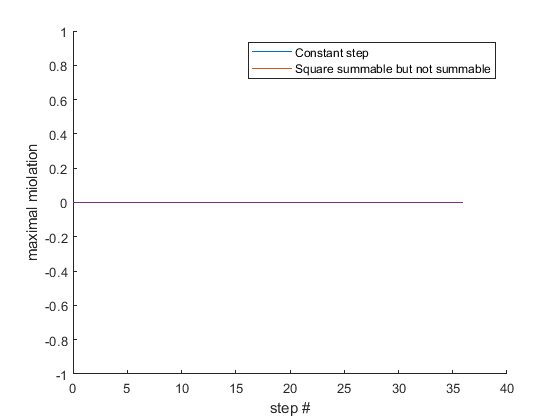
\includegraphics[width=\linewidth]{fig_3_1_2.png}
	\caption{Maximal violation for the linear constraints.}
	\label{fig:3_1_2}
\end{figure}



\section*{3.2 (4 points)} 
A randomized least squares solver. Consider the Least Squares minimization
problem
\begin{align*}
	\text{minimize } & \frac{1}{2 m} 
	\underbrace{\sum_{i = 1}^{m}
	(b_i - a_i^T x)^2}_{f(x)}
	\\
	\text{subject to } & x \in R^n \\
\end{align*}
where $a_1, \dots , a_m$ are rows of matrix $A.$
We will consider the stochastic
subgradient descent iterates
\begin{equation} \tag {1}
x^{t + 1} = x^t - \alpha_t g_t
\end {equation}
where $g_t$ is a noisy unbiased gradient of the objective function, i.e., $E[g^T|x^T] \in \partial f(x^t). $ \\

a) (1 point) Let  $j$ will be a random index chosen from 
$\{1, \dots, m\}$ such that for every index 
$i \in \{1, \dots, m\}$ the probability that $j = i$
is $p_i,$ i.e., 
$$
P(i = j) = p_i,
$$
for a given discrete probability distribution
$p_1, \dots, p_m \geq 0, $
$\sum_{i=1}^{m} = 1.$ 
Show that 
$$
E(\frac{(a_j^T x - b_j)}{m p_j} a_j) \in \partial f(x)
$$
where the expectation is taken over the random variable $j.$ \\

Solution: \\ \\

$$
f(x) = \frac{1}{2 m} (b - Ax)^T (b - Ax)
$$
The gradient of $f(x)$ is

$$
\frac{(A x - b)^T}{m} A
$$
or, component-wize
$$
e_i\frac{(a_i^T x - b_i)}{m} a_i
$$
there $e_i $  is the $i$-th component of the unit vector. \\
The expectation is
\begin{align*}
&E\frac{(a_j^T x - b_j)}{m p_j} a_j = \\
&\frac{1}{m} (E(a_j^T x - b_j) a_j / p_j)  = \\
&\frac{1}{m} (E(a_j^T x a_j / p_j) - E(b_ja_j / p_j))
\end{align*}

For the second member of equation:
\begin{align*}
E(b_j a_j / p_j)  = 
\sum_{j=1}^m e_j p_j b_j a_j / p_j = 
\sum_{j=1}^m e_j b_j a_j \\=  e_j b_j a_j.
\end{align*}	
there $e_j $  is the $j$-th component of the unit vector. \\
So, $ E(b_j a_j/p_j) = e_j b_j a_j.$ \\
The equality for the first member of the equation:
$$
E(a_j^T x a_j/p_j) = e_j a_j^T x a_j
$$
can be proved in the same way.
So, we're done. \\

(b) \\
Assume that $b = Ax*$ for some vector $x*$, i.e., 
$x \in arg \; min f(x).$ Define the error vector 
$e_t = x_t - x^*,$ where $x_t$ is the subgradient descent iterate in (1). Consider the the constant step size 
$\alpha_t = \frac{m}{||A||_F^2},$ the unbiased the unbiased subgradient from part
(a) sampled i.i.d. at every iteration, and the probability distribution
$$
p_i = \frac{||a_i||_2^2}{\sum_k ||a_k||_2^2} = \frac{||a_i||_2^2}{||A||_F^2}
$$

Show that the error vector $e_t$ obeys the time-varying linear dynamical system
$$
e_{t+1} = P_t e_t
$$
where $P_t$ is a (random) symmetric projection matrix, i.e., $P_t^T P_t = P_t^2 = P_t$ obeying 
$\mathbf{E}P_t = I - \frac{1}{||A||_F^2} A^T A.$\\

Solution: \\

\begin{align*}
& e_{t+1, j} = \\
& \text{(from (1))}\\
&x_{t,j} - \alpha_t g_{t,j} - x_j^* = \\
& e_{t, j} - \alpha_t g_{t,j} = \\
& \text{(using the equation for subgradient)}\\
& e_{t, j} - y_j \alpha_t (a_j^T x_{t,j} - b_j) a_j / mp_j = \\
& (\text{here } y_j \text{ is a random variable which is 
	equal either to 0 or 1 with probability } p_j)\\
& (\text{using the equation } e_t = x_t - x^*) \\
& e_{t, j} - y_j \alpha_t (a_j^T (e_{t,j} + x^*_j) - b_j) a_j / mp_j = \\
& (\text{as } a_j^T x^*_j - b_j = 0)\\
& e_{t, j} - y_j \alpha_t a_t^T e_{t, j} a_j / mp_j = \\
& e_{t, j}(1 - y_j \alpha_t a^T_j a_j / mp_j) = \\
& e_{t, j}(1 - y_j a^T_j a_j / (m * p_j ||A||_F^2) = \; \\ 
&(b1) \\
& \text{using the given expression for } p_j:\\
& e_{t, j}(1 - y_j a^T_j a_j / ||a_j||_2^2 = \\
&e_{t, j}(1 - y_j)
\end{align*}

If we rewrite the last equation in the matrix form 
we will get:

$$
e_{t + 1} = P e_t
$$
where $P = I - Y_j,$ where $Y_j$ is the matrix those
elements are equal $\delta_{ij} y_i, $ i.e., all non-diagonal elements are zero, and diagonal of matrix consists of the $y_i.$
This is evident that this matrix is a symmetric projection matrix, as 
$$
P = P^T, \; PP^T = P^2 = P.
$$ \\ \\
Using equation (b1) 
$$
e_{t + 1, j} = e_{t, i}(1 - y_j a_j^Ta_j/(m p_j ||A||_F^2))
$$
we get:
$$
P_{j, j} = (1 - y_j a_j^Ta_j/(m p_j ||A||_F^2))
$$
where $P_{j, j}$ is the $j, j-$ th element of matrix $P.$
then
$$
\mathbf{E}P_{j, j} = 1 - \sum_{i=1}^{m} p_j a_j^Ta_j/(m p_j ||A||_F^2) 
$$
i.e, 
$$
\mathbf{E}P = I - A^TA/||A||_F^2
$$
\\

(c) (1 point) Show that\\
$$
\mathbf{E}||e_{t+1}||^2_2 \leq 
\big(1 - \frac{\sigma_{min}(A)^2}{||A||_F^2}\big) E(||e_t||^2_2)
$$
where $\sigma_{min}(A)$ is the smallest singular value of $A.$ Hint: note that 
$
\mathbf{E}[||e_{t+1}||^2_2|e_t] = 
\mathbf{E} [e_t^T P_t^T P_t e_t |e_t] = 
\mathbf{E} [e_t^T P_t e_t |e_t] = 
e_t^T \mathbf{E}[P_t]e_t,$ and that 
$$
e^T A^T A e \geq \sigma_{min}(A)^2 e^T e.
$$
for every vector $e \in R^n.$ Apply this bound recursively to obtain a bound on $\mathbf{E}||e_{t}||^2_2,$ involving only $\mathbf{E}||e_{0}||^2_2,$ $||A||_F$, $\sigma_{min}(A).$









\end{document}